% !TEX root = Konzept.tex
\chapter{Game Design}
Da das technische Fundament bereits festgelegt wurde, machten wir uns zunächst genauere Gedanken zur Spielidee. Hierfür erstellten wir ein digitales Whiteboard bei Miro, um über einen einfachen und direkten Weg Ideen zu teilen und festzuhalten. Um hierbei die Wahl der Konzepte nicht bereits im Vorhinein zu stark einzuschränken, wurde eine sehr offene und erweiterbare Spielform, in Form eines \textit{Escape Rooms}, als Grundlage gewählt. Diese Idee wurde im Laufe der Entwicklung spezifiziert und stetig verändert, jedoch blieb erhalten, dass - ähnlich wie in einem Escape Room - ein Spieler Puzzle und Aufgaben verschiedener Arten lösen muss um das Ende zu erreichen. Dies bot die Freiheit mit vielen verschiedenen Ideen zu arbeiten, welche verschiedene Grundkonzepte der Interaktion ansprachen. Das finale Konzept der Spielidee lässt sich wie folgt beschreiben.
\section{Spielidee}
In einer magischen Welt, die zeitlich der Epoche des Mittelalters zuzuschreiben ist, sind auf mysteriöse Weise alle Farben verschwunden, da die Göttin der Farben ihrer Kräfte beraubt und in einem Turm eingesperrt worden ist. Indem ihr heiliges Diadem, welches die magischen Farbkristalle enthielt, zerbrochen wurde, hat nicht nur die Göttin ihre Kraft verloren, sondern alle Farben sind abhanden gekommen. Frei nach dem Motto \textit{Farben sind das Leben Lied}, existiert kein Leben ohne die entsprechenden Farben, weshalb ohne die Kristalle nichts korrekt funktioniert. Da jedoch ein Teil der Kraft der Göttin immer noch in den Kristallen gespeichert ist, geben diese genügend Farbe ab, um einen kleinen Bereich in gleichnamiger Farbe etwas Leben einzuhauchen. Sollte der Spieler die einzelnen Kristalle finden und ihre Kraft über eine Maschine wieder in ihre Umgebung einfügen können, so besteht doch noch etwas Hoffnung, um die Göttin aus dem Turm zu befreien.\\
\section{Setting/ Look \& Feel}
Der Look des Spiels orientiert sich, wie die Spielidee bereits vermuten lässt, optisch an einer magischen, rätselhaften Fantasy Welt, die durch viele bewegbare Treppen von den Treppenhäusern aus Harry Potter inspiriert wurde. Da die Farbkristalle im gesamten Turm verteilt sind, existieren neben der Farbe Weiß, nur noch die primären Farben des subtraktiven Farbschemas Cyan, Magenta, Gelb und Schwarz. Diese Farben sind, gemäß dem Hintergrund des Spiels, bereits zu Spielbeginn punktuell in verteilten Räumen zu finden. Das führt dazu, dass das Innere des Turms in separierte Bereiche unterteilt ist, wodurch die Orientierung dem Spieler im Laufe des Spiels deutlich einfacher fallen sollte. Jedem dieser Bereiche wurden eigene Themen zugewiesen, welche unserer Meinung nach am besten zur Farbe des Raums passen und eine flexible Auswahl an Rätselarten zulassen würden. Daraus ergaben sich folgende Räume, welche in einem späteren Kapitel nochmals genauer erklärt werden.
\newpage
\noindent
\subsection{Lobby}
Die Lobby symbolisiert den Bereich des Spiels, zu welchem der Spieler einige Male zurückkehren wird. Da dieser Raum an alle weiteren Farbräume grenzt, sollte er das Setting des Spiels als Ganzes aufgreifen. Somit ist die Lobby ein Raum, der mit magischen oder zur Herstellung magischer Objekte, wie Pflanzen und Erzen dekoriert ist. Zusätzlich zu diesem allgemeinen Magie-Thema, umfasst der Raum, vor allen durch das Minispiel/Rätsel des Raums, das Thema Alchemie, da man bei diesem Spiel Tränke braut.
\subsection{Cyan-Raum}
Der Cyan-Raum verkörpert als erster Farbraum des Spiels das Thema \dq Werkstatt\dq. In diesem Raum befinden sich nämlich üblichen Handwerksmaterialien, Konstrukte wie eine Uhr und Zahnräder, um ein Gefühl dafür zu bekommen, sich in einem Uhrwerk zu befinden. Hinzu kommt das Rätsel des Raums, bei welchem man Röhren an einer Wand befestigen muss. Hierbei soll dem Spieler erneut das Gefühl gegeben werden, dass dieser Raum zum Schaffen und Werkeln gedacht ist. Abgerundet wird der Raum durch eine dekorierte Golfbahn, um sich etwas von der Arbeit zu erholen.
\subsection{Magenta-Raum}
Im Magenta-Raum befinden sich neben Büchern und Leitern, große Tische. Diese Kombination von Objekten soll das Thema \dq Bibliothek\dq betonen. In diesem Raum befinden sich erstmals zwei Rätsel bzw. Minispiele. Im ersten Minispiel fordert es Geschick und Können, da der Spieler hier eine Murmel in einer Box durch Neigung in ein Loch navigieren muss. Allgemein ausgedrückt, stellt der Raum ein Studierzimmer dar, in welchem sich passenderweise Bücher und ein massiver Holztisch befinden. Dieser Tisch wird in einem zweiten Rätsel in Form eines Rätseltischs thematisiert.
\subsection{Dunkelraum}
Der letzte Raum des Spiels ist der Yellow-Room bzw. Dunkelraum. Um in diesem Raum für Abwechslung zu sorgen, fehlt hier die Beleuchtung fast vollständig, wodurch sich der angegebene Name ergeben hat. Die Thematik dieses Raums befasst sich aufgrund der Dunkelheit mit Astronomie, Astrologie und anderen Künsten. Mithilfe von Leuchtstäben muss ein Spieler hier selbst für Licht sorgen, um die Geheimnisse des Raums zu lüften und damit das Rätsel zu lösen.

\newpage
\noindent
\section{Spielbeginn}
\begin{wrapfigure}{r}{6cm}
	\vspace*{-0.5cm}
	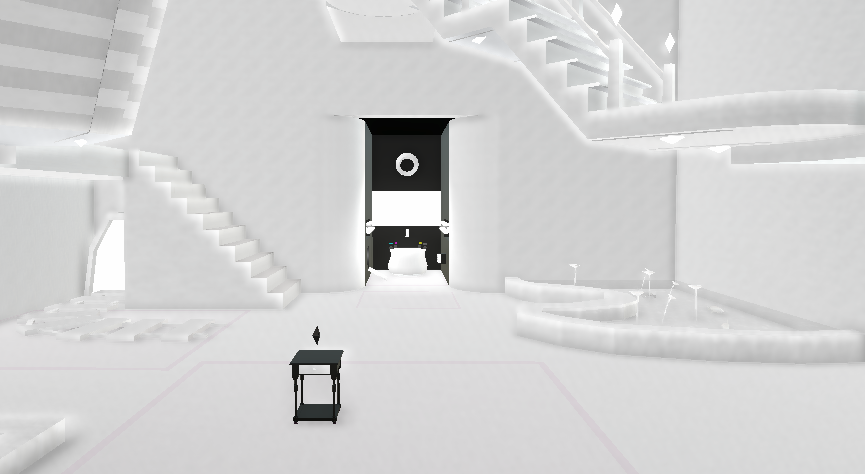
\includegraphics[width=5.9cm]{Pictures/Lobby_Start}
	\caption{Spielwelt zu Beginn}
	\vspace*{-0.5cm}
	\label{fig:spielwelt-beginn}
\end{wrapfigure}
Zm Spielbeginn befindet sich der Spieler bereits im Treppenhaus, welches den Hauptbereich des Spiels darstellt. Hier wird dem Spieler ein erster Eindruck vom Farbschema und der Größe des Turms gegeben. Sollte sich der Spieler etwas nach vorne bewegen, bekommt er zudem den ersten Kristall zu Gesicht, welchen er in gleicher Richtung auch direkt im ersten interaktiven Rätsel benutzen kann. Dazu aber in einem späteren Kapitel mehr.\\
\section{Spielfortschritt/Ziel}
Um im Spiel Fortschritt zu erzielen, muss ein Spieler die Rätsel der einzelnen Farbräume lösen und die daraus gewonnenen Farbkristalle im oben erwähnten Minispiel des Hauptraums, welcher im Folgenden als Lobby bezeichnet wird, in Farbe zu konvertieren, um so die verschiedenen Farben in die Spielwelt zurückzubringen.
Dabei ist zu beachten, dass die Räume auch nur dann erreichbar sind, sollte der Spieler die vorher abzuschließenden Rätsel abgeschlossen haben. An dieser Stelle wird eine besondere Spielmechanik relevant.
\subsection{Spielmechanik: Treppen}
\begin{wrapfigure}{r}{6cm}
	\vspace*{-0.5cm}
	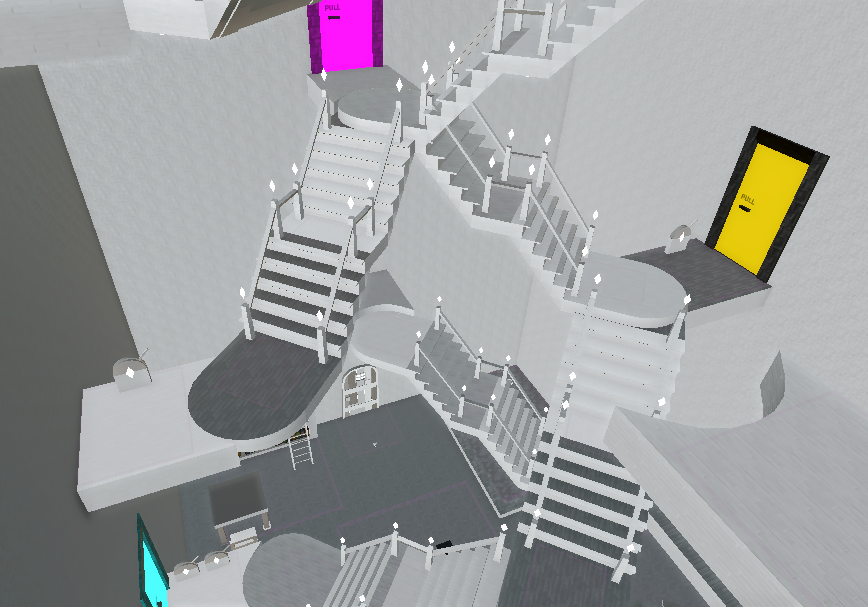
\includegraphics[width=5.9cm]{Pictures/Treppenhaus}
	\caption{Treppenhaus}
	\vspace*{-0.5cm}
	\label{fig:treppenhaus}
\end{wrapfigure}
Die Treppen der Lobby haben verschiedene Farben und nur wenn diese in die Welt zurückgebracht wurden, kann eine Treppe bewegt werden, um den Weg nach oben zu ermöglichen. Darüber hinaus zeigt sich in diesem Rätsel eine simplere Form des Interaktionskonzepts. Die Aktion des Ziehens eines farbigen Hebels führt direkt zu der Reaktion einer Auswahl gleichfarbiger Treppen, welche im Treppenhaus zu neuen Positionen rotieren. Hier zeigt sich die Stärke des Interaktionskonzepts in einer VR-Umgebung besonders, da ein Spieler nach dem Benutzen eines Hebels direkt um ihn herum die Auswirkungen dieser Aktion spürt. Weil bestimmte Kristalle für bestimmte Treppen zuvor eingesetzt worden sein müssen, bekommt das Spiel einen deutlich weniger linearen Spielverlauf, was uns besonders wichtig gewesen ist. Zusätzlich greift diese Spielmechanik das Interaktionskonzept mit der Umgebung zu interagieren auf, da sich die Welt direkt nach Betätigen des Hebels verändert.\\
\noindent Weiterhin wird ein Spieler im Verlauf des Spiels verschiedene Rätsel lösen und damit mehr Farben in eine zuvor fast ausschließlich weiße Welt einführen. Dieses Feedback bietet dem Spieler eine grobe Darstellung des Spielfortschritts, führt aber ebenso zu einem Gefühl von höherem Ziel und Zweck, ein Teil dieser Welt zu sein. Dies wird weiter dadurch verstärkt, dass die Rätsel des Spiels nur mit den richtigen Farben zu lösen sind und der Zweck somit nicht nur subtil in der Umgebung dargestellt, sondern spürbar in den darauffolgenden Rätseln verbaut ist.\newpage \noindent
\section{Bewegung im Spiel}
\begin{wrapfigure}{r}{6cm}
	\vspace*{-0.5cm}
	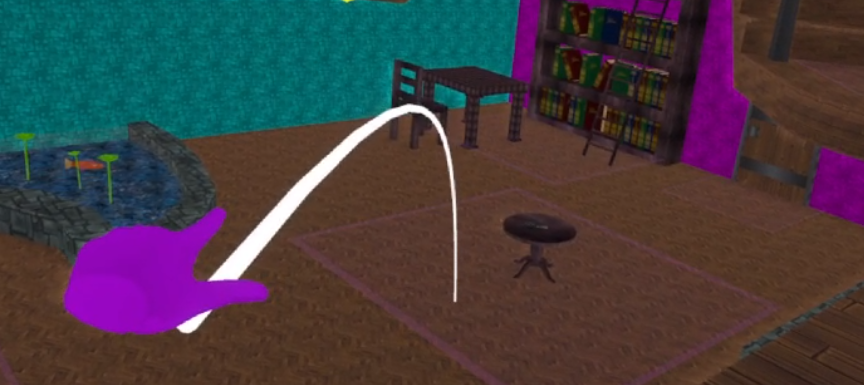
\includegraphics[width=5.9cm]{Pictures/Bewegung}
	\caption{Bewegung}
	\vspace*{-0.5cm}
	\label{fig:bewegung}
\end{wrapfigure}
Da dieses Projekt keinen Wert auf schnelle Bewegungen, sondern viel eher auf gute Spielerfahrungen und das Lösen von Rätseln ohne Zeitdruck legt, wurde sich für die Teleport-Fortbewegung und Snap-Drehungen entschieden. Außerdem sollte diese Entscheidung Motion Sickness erheblich vorbeugen. Zusätzlich wurden die Teleportationsbereiche bezüglich ihrer Anzahl deutlich reduziert, um die Bewegung des Spielers durch die jeweiligen Räume zu kontrollieren und somit sicherzustellen, dass ein Spieler die relevanten Bereiche eines Raumes erkennt und nicht allzu sehr von der Umgebung abgelenkt oder verwirrt wird. Ein Spieler hat somit die Möglichkeit mit dem Joystick der VR-Controller einen Laser zu erzeugen, welcher zunächst rot hervorgehoben wird. Sollte ein Laser das erste Mal in einen Teleportationsbereich hineingehalten werden, färbt sich dieser weiß. Das Loslassen des Triggers führt anschließend dazu, dass sich die Position des Spielers auf den Schnittpunkt zwischen Laser und Bereich setzen wird. Die einzige Ausnahme bilden hierbei die Teleportationsbereiche der Treppen. Sollte sich ein Spieler auf Treppenstufen teleportieren wollen, so ändert sich die Position abhängig vom Laser auf den nächstgelegenen Bereich der Treppe. Hierbei unterscheiden sich die Teleportationsbereiche hinsichtlich der neuen Position von Spielern nach der Teleportation. Während sich Spieler frei in einem Bereich positionieren können, ist die Position auf einer Treppe immer auf die Mitte des Bereichs beschränkt. Mehr dazu jedoch in einem späteren Abschnitt.

\section{Brainstorming: Weitere Spielideen}
Wie am Anfang dieses Kapitels erwähnt, sollte das Spiel eine offene Spielform innehalten, da in allen Formen von Entwicklungen bestimmte Prozesse und Umsetzungen mehr Zeit in Anspruch nehmen können, als man zuvor gedacht hat. Der Grundgedanke des Spiels wurde hierbei jedoch nicht verändert. In verschiedenen Rätseln innerhalb der Lobby und Farbräumen müssen die Kristalle durch das Lösen von diesen Rätseln erspielt werden, um das Spiel zu beenden. Da das Brainstorming jedoch ein wichtiger Bestandteil des Projekts war, sind hier kurz ein paar Informationen über nicht umgesetzte Ideen.
\subsubsection{Tippschalter}
Da es frustrierend sein kann, in Rätselspielen nicht voranzukommen und das Spiel entweder beiseite zu legen oder die Lösung über das Internet herauszufinden, war geplant in der Lobby einen Tippschalter zu implementieren, an welchem man Tipps ziehen kann, die dem Spieler einen Hinweis geben würden abhängig vom Fortschritt im Spiel.
\subsubsection{Farbhandschuh}
Zudem beschäftigten wir uns intensiv mit der Idee, wie die Farbe in das Spiel zurückkehren sollte. Ein Konzept war hierbei dies über einen Handschuh stattfinden zu lassen, welchen der Spieler in Sockets innerhalb der Wand steckt, um so die Farbe zurückzubringen. Zusätzlich sollte der Spieler hierbei in der Lage gewesen zu sein, mit seinen Fingern auf Oberflächen zu malen.
\subsubsection{Cyan-Raum}
Im Cyan-Raum wurde weiterhin geplant ein Angelspiel zu entwerfen, bei welchem der Spieler einen Gegenstand aus einem Brunnen fischen muss. 
Da sich im Cyan-Raum allerlei Ausrüstungs-gegenstände und Tools befinden, war zudem geplant, ein kleines Minispiel mit dem Bogen zu machen, mit welchem beispielsweise Farbballons zum Platzen gebracht werden sollten.
\subsubsection{Magenta-Raum}
Im Magenta-Raum sollte ein Timing-Minispiel entworfen werden bei welchem Leitern über Hebel so bewegt werden sollten, um über erhöhte Positionen versteckte Gegenstände zu erreichen.\\
Außerdem wollten wir eine Idee aus einem vorherigen Semester aufgreifen bei welchem ein Gegenstand so gedreht werden sollte, sodass dessen Schatten, der durch einen Scheinwerfer auf die Wand projiziert wurde, ein passendes Bild erzeugt. Abschließend wurde in geplant ein Bilderrätsel zu machen, welches in beispielsweise neun Segmente unterteilt ist, wobei diese entsprechend zum Original-Bild zurückverschoben werden sollten. 
\subsubsection{Dunkelraum}
Für den Dunkelraum wurde geplant, etwas Licht über einen leicht offenen Vorhang in den Raum zu lassen, welches auf einen Spiegel scheint. Mithilfe einer Konstellation aus Spiegeln sollte hierbei die Reflexion auf ein Ziel gelenkt werden.


\chapter{Umsetzung}
Doch was genau wurde letztendlich umgesetzt? In diesem Kapitel soll dies genauer erläutert werden.
\section{Alchemie-Puzzle}
\begin{wrapfigure}{r}{6cm}
	\vspace*{-0.5cm}
	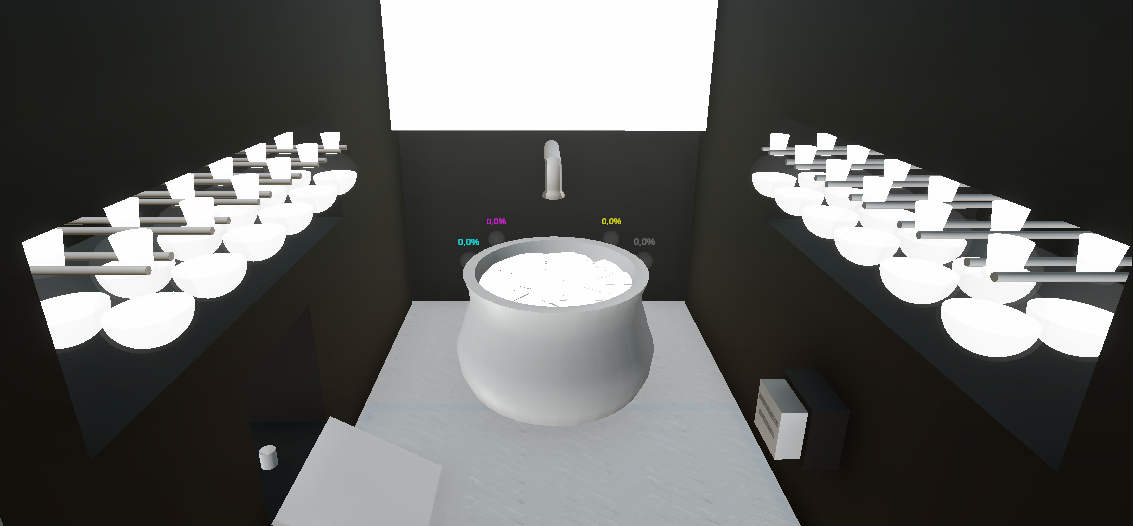
\includegraphics[width=5.9cm]{Pictures/Alchemie}
	\caption{Alchemie-Puzzle}
	\vspace*{-0.5cm}
	\label{fig:alchemie_start}
\end{wrapfigure}
Wie bereits in einem oberen Kapitel erwähnt, beschäftigt sich die Lobby mit dem Alchemie-Thema und bringt dabei ein Minispiel mit sich, welches der Spieler immer dann spielen wird, wenn er einen Kristall in die installierte Maschine platziert. Beim ersten Spieldurchgang hat der Spieler nur Zugriff auf die Farbe Weiß, womit man im Spiel nicht weit kommt. Da der Spieler den schwarzen Kristall in der Vorrichtung platziert hat, sieht der Spieler als Reaktion auf diese Aktion, dass die Maschine anfängt zu arbeiten, da aus ihr ein dampfartiger Partikeleffekt in Farbe des Kristalls ausgestoßen wird. Anschließend tropft eine schwarze Flüssigkeit in den Kessel, welcher sich vor der Maschine befindet. Diese färbt den Inhalt des Kessels schwarz ein. Um die genaue Farbe zu erkennen, befinden sich um den Kessel herum vier Textfelder, die den jeweiligen Farbwert im CMYK-Schema als Prozentwert mit zwei Nachkommastellen anzeigen. Als weitere Reaktion auf den platzierten Kristall aktiviert sich der Bildschirm auf Augenhöhe des Spielers. Dieser zeigt nun eine Farbe mit dazugehörigen CMYK-Farbwert analog zu den Werten, die sich um den Kessel befinden. Zusätzlich zur Startfarbe Weiß, verfügt der Spieler jetzt auch über die Farbe Schwarz. Mit diesen beiden Tränken kann er nun die Flüssigkeit des Kessels umfärben. Dabei erscheinen die Tränke auf der linken und rechten Seite des Bereichs über horizontale Schienen. Nimmt ein Spieler einen Trank, werden die anderen Tränke der Schiene so weiterbewegt und aufgestockt, als ob es schier unendlich viele gäbe. Den weißen Trank beispielsweise kann der Spieler anschließend in die Flüssigkeit werfen, um die auf dem Bildschirm abgebildete Farbe zu brauen. Technisch lässt sich das Färben folgendermaßen beschreiben: Die Farbe Schwarz hat für Cyan, Magenta und Gelb den Farbwert 0 und für Schwarz 100. Da Weiß überall den Wert 0 hat, wird anschließend von allen vier Werten der Mittelwert gebildet. Daraus resultiert also ein Grauton mit dem Schwarzwert 50.\\
\begin{figure}[h]
	\centering
	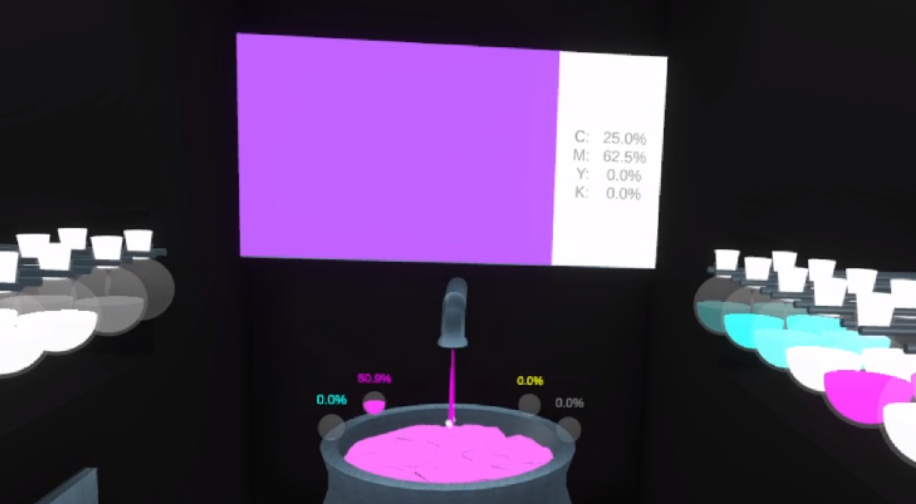
\includegraphics[width=\textwidth/2]{Pictures/Alchemie_Magenta}
	\caption{Alchemie-Puzzle Magenta}
	\label{fig:alchemie_magenta}
\end{figure}\newpage \noindent
Sollte ein Spieler das Gefühl haben, einen falschen Trank benutzt zu haben, so hat er die Möglichkeit das aktuelle Gemisch über einen Reset-Button auf der rechten Seite zurückzusetzen. Nach der Interaktion mit diesem wird nämlich die Farbe der Flüssigkeit im Kessel kurz weiß und anschließend mit der Farbe des Kristalls als Ausgangslage eingefärbt. Nachdem alle Etappen des Alchemie-Puzzles mit der Farbe Schwarz abgeschlossen wurden, schaltet sich der Bildschirm aus und es kommt erneut etwas gefärbter Dampf aus der Maschine. Weiterhin hat der Spieler jetzt Zugriff auf die Farbe Grau. Als Reaktion auf das abgeschlossene Rätsel färben sich alle Objekte, die einen schwarzen Farbton haben, in der Umgebung wieder so ein, wie sie üblicherweise wären. Zusätzlich sorgt dies dafür, dass die Interaktion mit gewissen Hebeln im Treppenhaus möglich ist. Da man im Spiel vier Kristalle findet, kann man dieses Minispiel bis zu vier mal spielen, bis man die gesamte Umgebung vollständig eingefärbt hat und das Endziel erreichen kann. Natürlich werden die Rätsel immer komplizierter, da dem Spieler immer mehr Farben zum Mischen zur Verfügung stehen. Hierbei sei gesagt, dass neben Schwarz, Weiß und Grau, die Farben Cyan, Magenta und Gelb in jeweils einer helleren und dunkleren Variante existieren werden.
\begin{figure}[h]
	\centering
	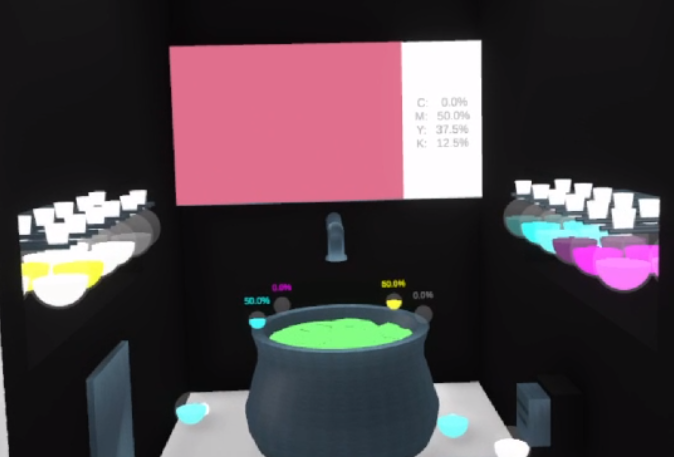
\includegraphics[width=\textwidth/2]{Pictures/Alchemie_Final}
	\caption{Alchemie-Puzzle Gelb}
	\label{fig:alchemie_final}
\end{figure}\newpage \noindent

\section{Röhren-Puzzle}
Nachdem ein Spieler das erste Alchemie-Rätsel absolviert hat, ist er in der Lage den Cyan-Raum zu erreichen. In diesem befindet sich eine Vorrichtung aus ein paar wenigen Röhren. Durch eine leichte transparente Gitter-Struktur in der Wand soll dem Spieler vermittelt werden, dass herumliegende Röhren in dieser zu platzieren sind. Die Objekte befinden sich beim ersten Berührungspunkt mit dem Spieler in einer Kiste, aus welcher sie dann aufgehoben werden können. Da Anfang und Ende des Puzzles bereits fest installiert sind, sollte der Spieler eine Auffangschale rechts neben dem Start bemerken. In der Nähe dieser wird über einen Hinweis bereits angedeutet, dass hier ein Gegenstand empfangen werden kann. Beim genaueren Verfolgen der Röhren sollte man schlussfolgern, dass sich der blaue Kristall in den waagerechten Röhren oberhalb des Spielers befindet. Um ihn zu erreichen muss man also einen Durchfluss ermöglichen. Dazu hat man jedoch nur begrenzt viele Rohre. Diese lassen sich dabei in zwei Kategorien mit je zwei Variationen unterscheiden. In der Vorrichtung befinden sich nämlich gewinkelte, sowie gerade Röhren, welche frei bewegt und platziert werden können. Hinzu kommen bereits fest installierte, welche lediglich hinsichtlich ihrer Rotation angepasst werden können. Dies wird dem Spieler über Rotationspfeile auf den Gegenständen präsentiert. Wenn eine Röhre in die Gitterstruktur gehalten wird, erscheint dem Spieler eine transparente und korrekt positionierte Preview der Röhre an welcher sie platziert werden würde, sollte man sie loslassen. Die Preview hat dabei eine von vier möglichen Rotationen, welche anhand der Rotation des Rohrs ermittelt wird. Jedes Mal, wenn eine Röhre platziert wurde, nimmt eine Röhre die Position und Rotation der zuvor sichtbaren Preview ein. Weiterhin prüft der Manager des Rätsels, ob das Ende der Röhren vom Start ausgegangen ohne Lücken erreicht werden kann. Dabei schaltet sich bei allen Röhren, welche den weiteren Durchfluss gewährleisten, ein Licht an, um dem Spieler Feedback darüber zu geben, ob er die Verbindung richtig gesetzt hat. Technisch betrachtet lässt sich sagen, dass ein Rohr in diesem Spiel bis zu zwei Nachbarn haben kann, welche über Collider gesetzt werden können. Somit lässt sich die Iteration über platzierte Röhren als verkettete Liste betrachten, da ein Rohr seine Nachbarn kennt. Der Trick an diesem Rätsel ist die Begrenzung der Möglichkeiten durch die feste Anzahl an zu platzierenden Röhren und der Variation aller zuvor platzierten Rohre, welche lediglich rotiert werden können. Dadurch ergibt sich nach genaueren Überlegungen anhand gegebener Mittel eine einzige Lösung zu welcher man nur durch Überlegen und Ausprobieren kommt.\\
Sollte der Durchfluss vollständig sein, aktiviert sich theoretisch betrachtet die Farbe im Rohr-system, wodurch die Farbe den Kristall herausströmt.
\begin{figure}[h]
	\centering
	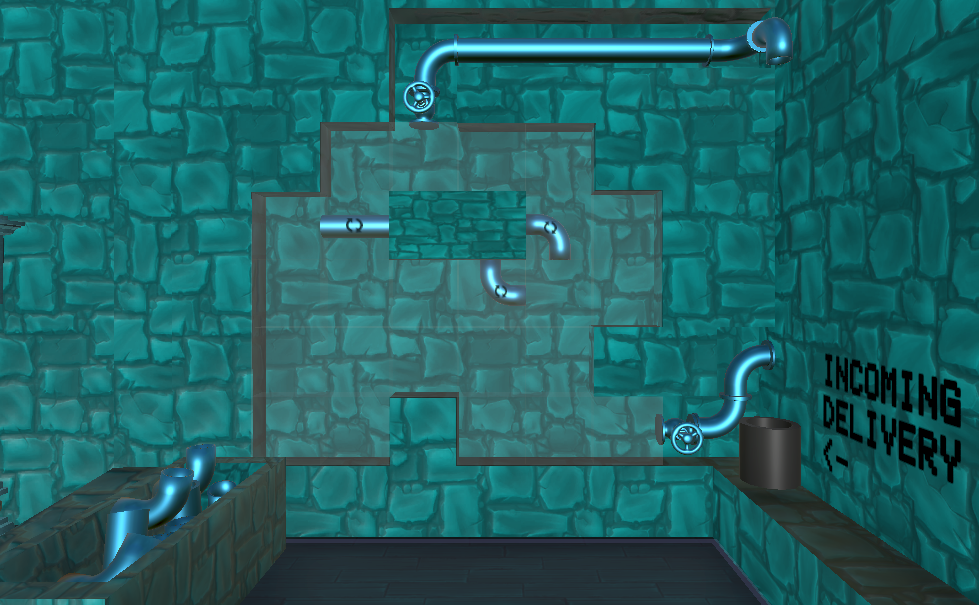
\includegraphics[width=\textwidth/2]{Pictures/Roehren}
	\caption{Röhren-Puzzle}
	\label{fig:cyan}
\end{figure}\\
\section{Murmelbox}
Der daraufhin freigeschaltete Magenta-Raum enthält wie zuvor erwähnt, u.a. eine Murmelbox. Diese Box enthält, wie der Name bereits vermuten lässt, eine Murmel, welche zur Lösung des Spiels in das Loch befördert werden muss, welches sich im Mittelpunkt der Box befindet. Die anderen Löcher der Box führen hingegen dazu, dass die Kugel in ihre Ausgangslage zurückversetzt wird. Bestimmte Löcher können hierbei dazu beitragen, dass zuvor versperrte Wege, frei werden, um den Schwierigkeitsgrad des Spiels etwas zu verringern. Außerdem befinden sich in der Box farblich gekennzeichnete Druckplatten an einigen Stellen, welche optisch hervorgehobene um das zentrale Loch sich befindende Wände herunter- oder hochfahren. Dabei wurde die Box so konzipiert, dass man die Kugel nicht zu schnell rollen lassen darf, dass eine Druckplatte hierbei die sich auf der anderen Seite befindende Wand herunterfahren würde, wodurch die Murmel auf einer weiteren landet, welche die Wand erneut hochfährt. Das mag bei manchen Spielern vermutlich für etwas Frustration, gleichzeitig aber auch Ehrgeiz sorgen.\\
\begin{wrapfigure}{r}{6cm}
	\vspace*{-0.5cm}
	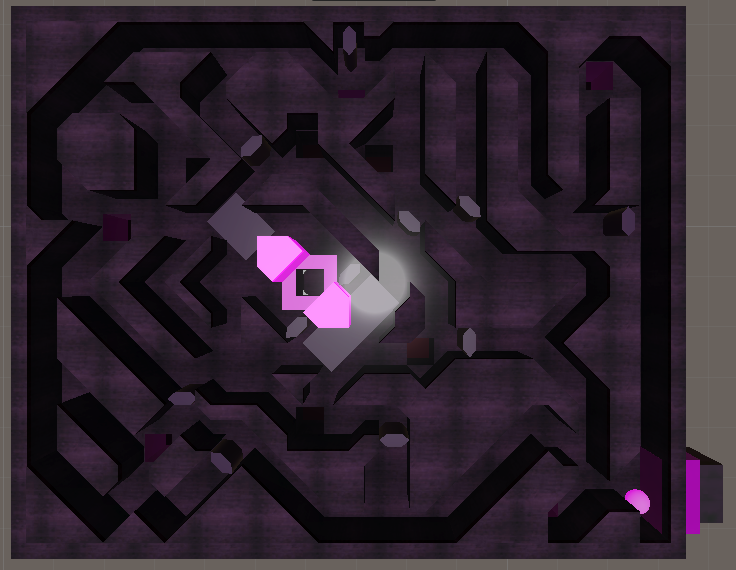
\includegraphics[width=5.9cm]{Pictures/Murmelbox}
	\caption{Murmelbox}
	\vspace*{-0.5cm}
	\label{fig:murmelbox}
\end{wrapfigure}
Die Murmelbox lässt sich dabei allgemein ausgedrückt mittels zweier Hebel bewegen. Der linke verstellt hierbei bei einer Neigung nach links oder rechts die Rotation der Box in die entsprechende Richtung. Der rechte Hebel lässt die Box analog durch Neigungen nach vorne und hinten rotieren. Diese Steuerung erfordert einiges an Geschick, Geduld und Multitasking-Fähigkeiten, u.a. da sich das Gehirn erst auf diese einstellen muss. Schafft es der Spieler die Kugel in das Loch zu navigieren, schaltet sich das Lampenlicht über der Box aus, um zu signalisieren, dass das Rätsel geschafft ist.
\section{Rätseltisch}
Zusätzlich zur Murmelbox enthält der Magenta-Raum einen Rätseltisch, der etwas einem Sekretär ähnelt. Der Spieler kann sich dabei frei um den Tisch herumbewegen, um ihn vollständig prüfen zu kennen, da dieser, wie der Name bereits erschließen lässt, zum Rätseln anregt. Insgesamt vier Rätsel sind in diesem Tisch verbaut, wobei sich das vierte aus der Lösung vorheriger erst vollständig freischaltet.
\subsection{Part 1}
\begin{wrapfigure}{r}{6cm}
	\vspace*{-0.5cm}
	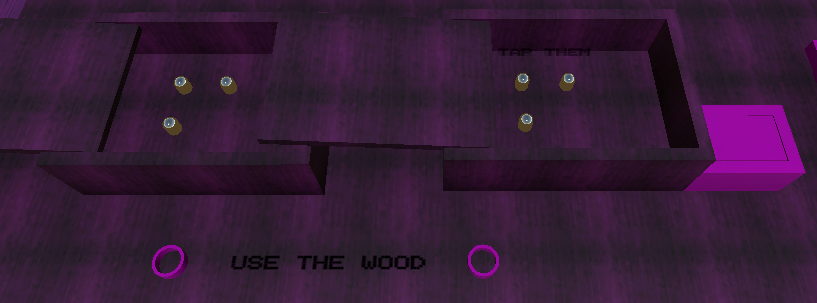
\includegraphics[width=5.9cm]{Pictures/Tisch1}
	\caption{Rätseltisch 1}
	\vspace*{-0.5cm}
	\label{fig:tisch1}
\end{wrapfigure}
Das erste Rätsel des Tischs enthält zwei nebeneinander liegende Kisten und jeweils eine Vorrichtung in welche man einen Finger stecken kann. Steckt ein Spieler einen davon in das Loch, öffnet sich die Klappe der zugeordneten Kiste nach links. In jeder Kiste befinden sich ausgeschaltete Lichter, welche durch eine Berührung mit der Hand wieder an- und ausgeschaltet werden können. Zieht der Spieler den Finger aus dem Loch, gehen die Lichter aus und die Klappe schließt sich wieder. Wie also schafft es der Spieler alle Lampen anzumachen ohne, dass sich eine der Klappen schließt? Um diese Frage zu beantworten, sollen Spieler den Hinweis zwischen beiden Fingerlöchern lesen. Aus diesem ergibt sich, dass im Raum ein Holz existiert, dass zum Blockieren genutzt werden kann. In einer Ecke des Raums befindet sich ein abgebrochenes Tischbein, welches man hierzu nutzen kann. Nachdem alle Lichter aktiviert worden sind, öffnet sich ein kleines Schächtelchen. In diesem befindet sich ein Papier auf dem der Buchstabe P abgebildet ist, das zur Lösung des finalen Rätsels benötigt wird. 
\subsection{Part 2}
\begin{wrapfigure}{r}{6cm}
	\vspace*{-1cm}
	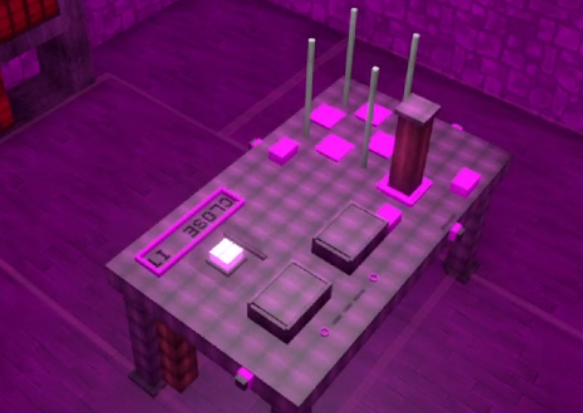
\includegraphics[width=5.9cm]{Pictures/Tisch2}
	\caption{Rätseltisch 2.1}
	\vspace*{0cm}
	\label{fig:tisch2}
\end{wrapfigure}
Für das zweite Rätsel erfordert es etwas Hand- und Augen-Koordination. Auf der rechten Seite des Tischs befindet sich eine Säule mit einem Ring darum, auf welchem geschrieben steht, dass dieser gegriffen werden kann. Sollte man den Ring greifen und nach oben ziehen, setzt er sich in festen Positionen fest. Doch diese Aktion erfüllt noch keinen Zweck. Damit er einen Nutzen hat, muss ein Spieler den sich davor befindenden Knopf drücken. Das würde dazu führen, dass die Farbe in der Säule steigt. Lässt man den Knopf los, nachdem man den Ring auf die erste Position gezogen hat, bleibt die Markierung an der Säule bestehen. Ansonsten sinkt diese wieder auf den Anfang. Zieht man den Ring also nach oben ohne das ein Finger einen Knopf betätigt, sinkt der Ring. Mit diesem Wissen, sollten Spieler nach der Erkundung des Tischs auf die Idee kommen, dass sie die vier Knöpfe nacheinander drücken müssen und zwischendurch den Ring auf die erhöhten Positionen stellen, um den Zwischenstand zu behalten. Sobald die Säule vollständig eingefärbt ist, öffnet sich eine zweite Schachtel, in welcher sich ein weiteres Papier mit dem Buchstaben N befindet.
\subsection{Part 3}
\begin{wrapfigure}{r}{4cm}
	\vspace*{-1cm}
	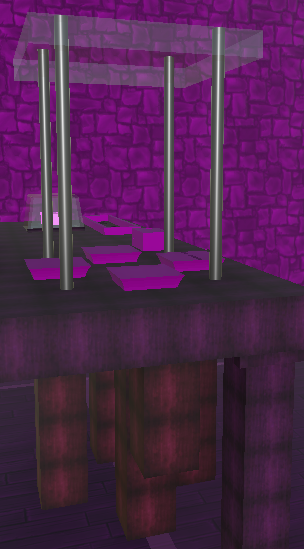
\includegraphics[width=4cm, height=6cm]{Pictures/Tisch3}
	\caption{\\ \noindent Rätseltisch 3}
	\vspace*{-1cm}
	\label{fig:tisch3}
\end{wrapfigure}
Im dritten Rätsel muss man ähnlich zum zweiten, Dinge greifen und nach oben ziehen. In der Nähe des vorherigen Rätsels befinden sich vier Pfähle , welche gleichmäßig in einem Kreis angeordnet sind. Hierbei können die Holzpfähle nicht aus dem Tisch gezogen werden, da sie durch eine sich auf dem Rätsel befindende Glasscheibe in ihrer Bewegung nach oben beschränkt sind. Für die Lösung des Rätsel muss man einen Blick unter den Tisch werfen. Hier sind Teile der Pfähle bereits zu sehen. Ziel ist es, dass ein Pfahl so weit nach oben gezogen wird, dass sein Bestandteil unterhalb des Tischs die gleiche Tiefe besitzt wie der unveränderbare Part daneben. Wenn alle vier Pfähle die korrekte Höhenstellung haben, öffnet sich die letzte Schachtel mit einem leeren Papier.
\subsection{Finales Rätsel}
\begin{wrapfigure}{r}{4cm}
	\vspace*{-0.5cm}
	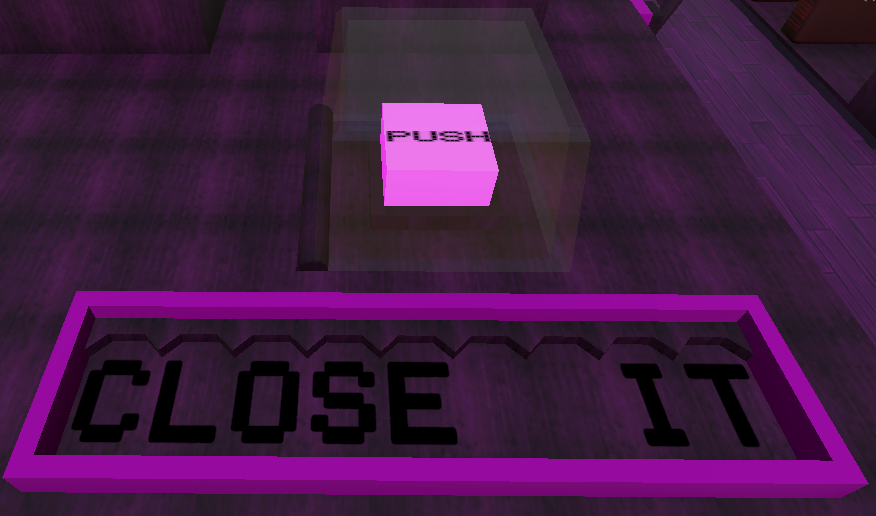
\includegraphics[width=4cm]{Pictures/Tisch4}
	\caption{\\ \noindent Rätseltisch Finale}
	\vspace*{-1.5cm}
	\label{fig:tisch4}
\end{wrapfigure}
Für den letzten Part des Rätsels muss sich der Spieler auf die andere Seite des Tischs begeben. Hier befindet sich ein Knopf mit einer Glaskapsel darum. Davor steht mit einzelnen Buchstaben \dq CLOSE  IT\dq. Da ein weiteres Leerzeichen vor dieser Wortkombination angelehnt ist, ergibt sich die Schlussfolgerung, dass das Wort geändert werden kann. Durch die zwei verfügbaren Leerzeichen, sowie die Buchstaben P und N, muss ein Spieler den Textinhalt so verändern, dass sich die Kapsel buchstäblich öffnet. Dazu hat er die zwei Leerzeichen auf die ersten Buchstaben von Close, sein P auf das S und sein N auf das erste Leerzeichen zu legen. Daraus resultiert die Wortkombination \dq OPEN IT\dq, was die Box öffnet. Nachdem der sich darin befindende Knopf betätigt wurde, schaltet sich das Licht des Tischs aus und der Kristall erscheint hinter dem Spieler in einem sich öffnenden Buch.
\noindent
\section{Dunkelraum}
\begin{wrapfigure}{r}{8cm}
	\vspace*{-0.5cm}
	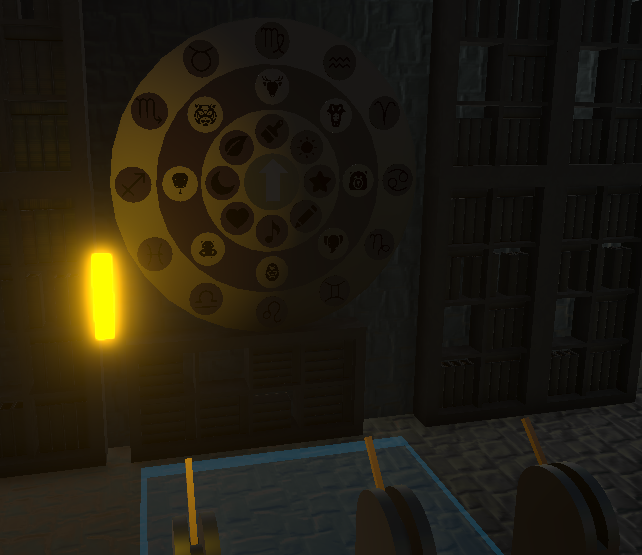
\includegraphics[width=8cm]{Pictures/Dunkelraum}
	\caption{Dunkelraum}
	\vspace*{-0.5cm}
	\label{fig:dunkelraum}
\end{wrapfigure}
Im letzten Farbraum des Spiels, dem Dunkelraum, wird dem Spieler die Fähigkeit normal zu sehen, entzogen. Mithilfe eines leuchtenden Spenders, den ein Spieler im Raum durch das starke Leuchten finden wird, kann man den Raum durch greifbare Leuchtstäbe punktuell erhellen und erforschen. Das wird auch für die Lösung des Raums benötigt. Wie bereits in einem vorherigen Kapitel erwähnt, sind die Themen des Raums Astronomie, Astrologie, Mystik und Kunst. Diese Themen tragen zusammen zur Lösung eines verstellbaren Rads bei, welches in drei Sektionen unterteilt ist. Der äußere Ring zeigt hierbei die Symbole der zwölf Sternzeichen. Abgesehen von dem Spender und seinen Leuchtstäben leuchtet lediglich ein Sternbild an der Decke, welches eins dieser zwölf Sternzeichen darstellt. Um dem Sternbild ein Zeichen zuordnen zu können, muss man im Raum eine Legende finden, die diese Beziehung aufweist. Das mittlere Segment des Rads umfasst acht Tiere, u.a. Hirsch, Tiger, Nilpferd und Bär. Alle diese vier Tiere befinden sich in Form eines Kopfes als Trophäe im Raum wieder. Um die richtige Lösung zu finden, muss man die Tierköpfe mit den Leuchtstäben gründlich erforschen, da auf der Rückseite eines Kopfes das richtige Symbol versteckt ist. Dies mag zu Beginn etwas unscheinbar sein, jedoch handelt es sich bei diesem Spiel um ein Rätsel-Spiel und die Tierköpfe sind allesamt erreichbar und auf dem Rad zu finden. Daher sollte es naheliegend sein, zu versuchen mit ihnen zu interagieren. Das letzte Segment des Rads umfasst acht verschiedene Symbole, die teilweise Anlehnungen an Namen von Tarotkarten sind. Sollte sich der Spieler im Raum gründlich genug umschauen, so findet er ein Schränkchen mit einer Schublade in welcher sich zuzüglich zu einem Buch eine Tarotkarte befindet. Dessen Name lässt auf das korrekte Symbol auf dem Rad schließen. Wenn der Spieler nun mittels Hebel die drei Segmente auf ihre richtige Position bzw. Rotation bringt, leuchtet der Pfeil des Rads hell auf und eine versteckte Wand öffnet sich, sodass der darin liegende Kristall aufgesammelt werden kann.
\begin{figure}[h]
	\centering
	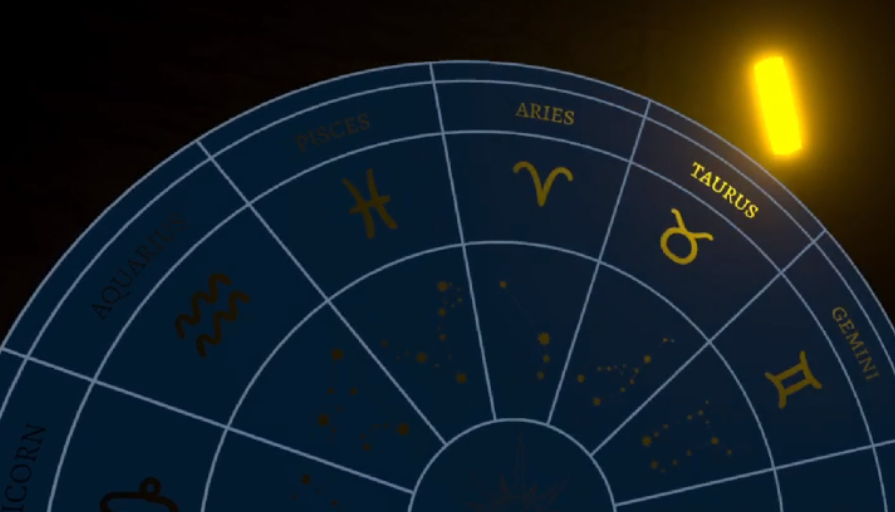
\includegraphics[width=\textwidth/3, height=3cm]{Pictures/Dunkelraum_Sternenkarte}
	\caption{Sternenkarte}
	\label{fig:dunkelraum_sternenkarte}
\end{figure}\newpage \noindent
Wie zuvor erwähnt, ist die Einschränkung der Sicht auch ein gutes Mittel, um besondere Erfahrungen mit visuellen Interaktionen zu sammeln, da der Raum die Verantwortung der Sicht auf den Spieler legt. Im Dunkelraum, muss er Lichtquellen in den Raum werfen, um die allumfassende Dunkelheit des Raumes punktuell zu durchbrechen. So etwas fundamentales wie die Lichtverhältnisse eines Raumes in die Hand der Spieler zu legen, führt zu einer deutlichen Erhöhung der Konzentration und Immersion. Dabei fiel auf, dass Spieler, die damit beschäftigt waren ihren Sichtsinn aufrechtzuerhalten, intensiver in das Spiel vertieft waren.
\section{Spielabschluss}
\begin{wrapfigure}{r}{6cm}
	\vspace*{-0.5cm}
	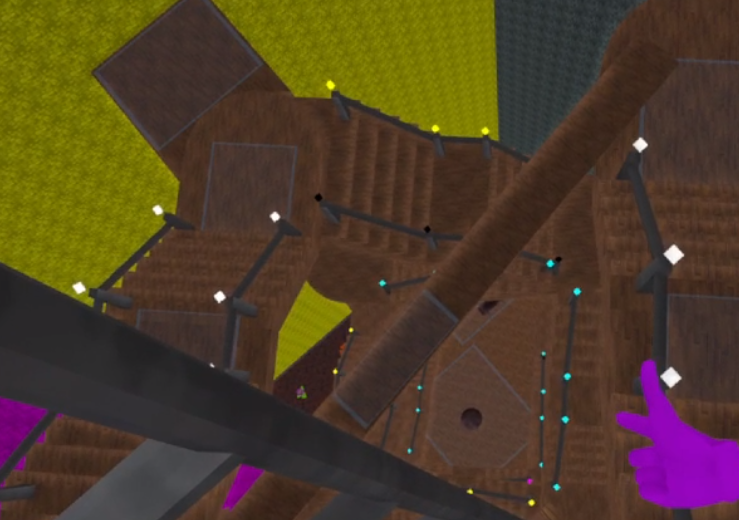
\includegraphics[width=5.9cm]{Pictures/Ausblick_Leiter}
	\caption{Ausblick Leiter}
	\vspace*{-0.5cm}
	\label{fig:leiter}
\end{wrapfigure}
Um das Spiel abzuschließen, muss der Spieler zuvor alle der vier Farbkristalle gefunden und mithilfe des Alchemie-Puzzles aktiviert haben. Damit ist er in der Lage alle Hebel des Treppenhauses zu nutzen, sodass die oberste Etage des Turms erreicht werden kann. Hier, beim höchsten Punkt des Turms, wird der Spieler vor eine weitere interessante, visuelle Interaktion gestellt. Er muss auf eine dünne Planke steigen, wobei man ein freies Sichtfeld auf die Tiefe unter sich hat. Die Reaktion auf diese Höhe kann sehr individuell sein, jedoch erzeugt sie starke Emotionen.\\
Anschließend muss der Spieler eine lange Leiter hochzuklettern, um den silbernen Schlüssel zu erlangen. Nachdem er diesen aufgesammelt hat, kann er in die Lobby des Turms zurückkehren und den gefundenen Schlüssel in die Eingangstür zu stecken. Um die Tür jedoch zu öffnen, erfordert es weiterhin eine Drehung, was erneut für eine stärkere Immersion des Spielers sorgt. An dieser Stelle erscheint ein Endbildschirm, welcher das Spiel beendet.
\begin{figure}[h]
	\centering
	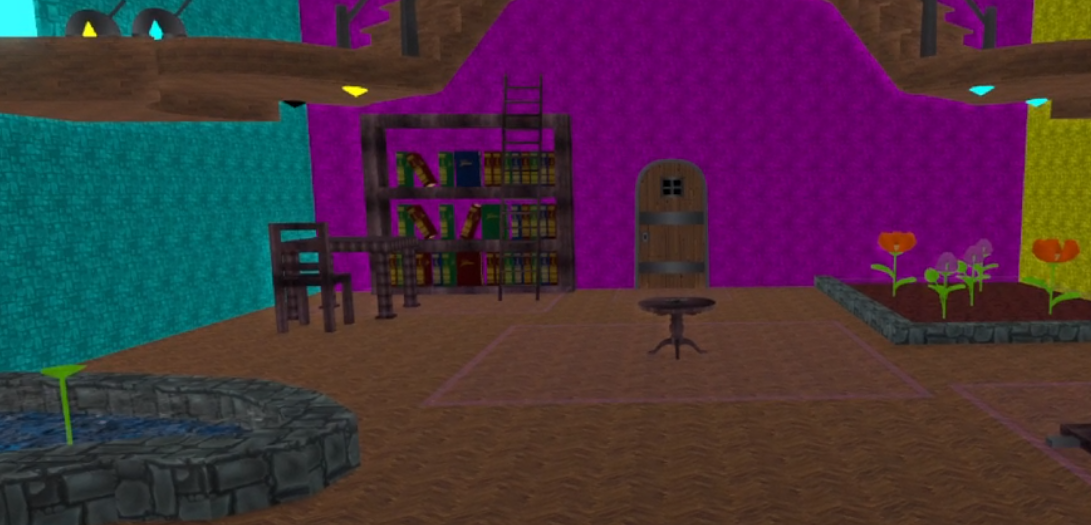
\includegraphics[width=\textwidth/2]{Pictures/Lobby_Final}
	\caption{Lobby Spielende}
	\label{fig:lobby_final}
\end{figure}